\documentclass[mathserif,10pt%,ps2pdf
]{beamer}
\hypersetup{pdfpagemode=FullScreen}
%\usepackage{amsmath, amsfonts, amsbsy, pstricks, pst-node, pst-text, pst-3d}
\usepackage{pst-plot, pstricks,pstricks-add,pst-node, pst-tree}
\usepackage{fancybox,amssymb,color}
\usepackage[latin1]{inputenc}
\usepackage{graphicx}
\usepackage{epsfig}
%\usepackage{natbib}
\usepackage{enumerate}
\usepackage{float}
\usepackage{pifont}
\usepackage{wasysym}
\usepackage{marvosym}

\beamertemplatenavigationsymbolsempty
%\setbeameroption{show notes}
%\setbeamerfont{caption}{size=\tiny}

\mode<presentation>
{
\usetheme{Singapore}
}

\title{Generation Capacity Investment in Oligopolistic Electricity Markets under Uncertainty}
%\subtitle{Peak Load Pricing under Imperfect Competition and Price Caps}


\author[Anton Burger and Robert Ferstl]{Anton Burger\inst{1} \hspace{2cm} Robert Ferstl\inst{2}}
\date[IAEE, June 18-20, 2008]{\small International Association for Energy Economics\\Istanbul, Turkey\\\vspace{0.3cm}\emph{June 18-20, 2008}}


\institute[Universities Vienna and Regensburg]{
\inst{1}Research Institute for Regulatory Economics\\
Vienna University of Economics and Business Administration, Austria
\and
\inst{2}Department of Finance\\
University of Regensburg, Germany}

%\institute{\includegraphics[scale=0.6]{N:/Institut/Regulierungsoekonomie/Institutslogos/RI_blau_kl.pdf}
%}

%\logo{\includegraphics[scale=0.45]{N:/Institut/Regulierungsoekonomie/Institutslogos/wulogo.pdf}
%}

\begin{document}

\maketitle

\begin{frame}{Outline}
\tableofcontents
\end{frame}

\section{Motivation}
\subsection{Motivation}

\begin{frame}{Motivation}

\begin{itemize}
	\item electricity markets are liberalized
	\item profit maximizing players instead of central capacity planning 
	\item \textbf{decentralized} market decisions
\end{itemize}	

there are qualms about adequacy of investments
	
\begin{itemize}
	\item california blackouts
	\item nuclear phase out in germany
	\item aging capacities throughout Europe and the US
\end{itemize}

\end{frame}
\subsection{Problem Structure}

\begin{frame}{Basic Structure of the Investment Problem}

\begin{itemize}
	\item How might the world change?
\begin{itemize}
  \item optimization under uncertainty
	\item demand uncertainty?
	\item increased demand volatility (wind)
	\item input costs (CO2 and Oil prices)
\end{itemize}

  \item How will the other players react?
  
\begin{itemize}
	\item Game Theory
	\item Cournot - Nash equilibriua
	\item the players are big: Herfindal Hirschmann Index $>$ 2000
\end{itemize}
\end{itemize}

\begin{itemize}
	\item inherently two stage setting
	
\begin{itemize}
	\item It takes a long time to build capacities but production quantities can be varied in the short run
	\item limited storage of electricity - L-shaped cost function - scarcity rents
\end{itemize}
\end{itemize}

\end{frame}
\subsection{Literature and own Contribution}


\begin{frame}{Literature}

\begin{itemize}
	\item welfare optimal prices and capacities under volatile/uncertain demand - Peak Load Pricing \cite{Crew1986}
	\item capacity decisions prior to Bertrand competition \cite{Kreps1983}
	\item capacity decisions under uncertainty prior to Cournot competition \cite{Gabszewicz1997}
\end{itemize}

\begin{itemize}
	\item calibrated numerical models of electricity markets \cite{Genc2007}, [Gabriel and Zhuang (2008)]
	\item based on Mixed Complementarity Problem (MCP) formulations \cite{Ferris2000}
\end{itemize}

\end{frame}

\begin{frame}{Two Contributions}

\begin{itemize}

\item theory - Peak Load Pricing under Imperfect Competition and Price Caps	

\begin{itemize}
  \item setup similar to \cite{Gabszewicz1997} but formulation as discrete time Hamiltonian
	\item nice interpretation of shadow prices
	\item simpler notation
  \item compare different market forms
  \item price cap restrictions
\end{itemize}

\item empirical / numerical - How will firms on a real market behave?

\begin{itemize}
	\item calibration with real data
	\item numerical solutions 
	\item multistage scenarios ................ ROB noch adden
\end{itemize}

\end{itemize}
\end{frame}


\section{Model}
\subsection{Assumptions}

\begin{frame}{Assumptions}

\begin{itemize}
	\item There are 1, $N$ or $\infty$ players

	\item price rationing is possible
	\item willingness to pay of buyers on the wholesale market = willingness to pay of final customers
	\item linear variable costs $c$ and capacity constraints
	\item $\alpha^s-\beta Q^{s,t}$ whereby $Q^{s,t}= \sum_{i\in I} q_{i}^{s,t}$
\begin{itemize}
	\item linear demand
	\item different $\alpha^s$ depict uncertainty ($s\in S$ scenarios)
	\item $\alpha^l > c + \Gamma$ quantities are always positive
\end{itemize}
	\item two points in time $t\in 0,1$ - investment, market equilibrium
\end{itemize}
\psset{unit=1.0cm} 
  \begin{pspicture}(-1,0)(8,2)
  %\showgrid
  \tiny
  \textcolor{red}{
  \psline[linecolor=red]{>->}(0,1)(7,1)
  \multido{\rA=0.5+1.5,\iB=0+1}{4}{
  \rput(\rA,1.9){$\iB$}
  \psline[linecolor=red]{->}(\rA,1.8)(\rA,1.2)
  \psline[linecolor=red](\rA,1.1)(\rA,0.9)
  }
  \rput(7.5,1){Zeit}
  \uput{0.2}[-90](0.5,1){\parbox{1cm}{ regulator sets price cap}}
  \uput{0.2}[-90](2,1){\parbox{1cm}{firms invest $t=0$}}
  \uput{0.2}[-90](3.5,1){\parbox{1cm}{uncertainty is realized (Nature)}}
  \uput{0.2}[-90](5,1){\parbox{1cm}{market equilibrium \\ $t=1$}}
 % \uput{0.2}[-90](6.5,1){\parbox{1cm}{Der Vertrag wird exekutiert}}
  }
  \end{pspicture}

\end{frame}

\subsection{Maximization Problem of one Player I}

\begin{frame}{Maximization Problem of one Player}

\begin{gather}
	\max \pi_i(q_{i}^{s,t},K_{i}^t,I_{i}^t)=
	\sum_{s\in S} \rho_s \left[ ((\alpha^s- \beta Q^{s,1}) - c) q_{i}^{s,1}  \right] - \Gamma I_{i}^{0} \label{eq:oligopmax2} \\
			\text{s.t.:} \  q_{i}^{s,1} - K_{i}^t \leq 0; \ \forall i,s \label{eq:capacitycon} \\ 
										  K^{1}_{i}  - K^{0}_{i}  - I_{i}^0 = 0 ; \ \forall i  \label{eq:state} \\
										   q_{i}^{s,1}; K^t_{i}; I_{i}^0	\geq 0; \ \forall i,s,t  \nonumber
\end{gather}

{\small
\begin{tabbing}
whereby: \= $\rho_s$ \= probability for scenario /  market state\\
\> $I_{i}^{0}$     \>   investments - action variable  \\
\> $K_{i}^t $      \>   capacity - status variable \\
\> $\Gamma$        \>   investment costs \\
\> $c$             \>   short run marginal costs \\
\end{tabbing}}
\end{frame}

\begin{frame}{Maximization Problem of one Player II}

corresponding discrete time Hamiltonian:

\begin{gather}
	 H_i(q_{i}^{s,t},K_{i}^t,I_{i}^t,\lambda_{i}^{s,1},u_{i}^1)= 
	 \sum_{s\in S} \rho_s \left[((\alpha^s- \beta Q^{s,1}) - c) q_{i}^{s,1} \right]	- \Gamma I_{i}^{0}  \\ \nonumber  
	  	- \lambda_{i}^{s,1}(q_{i}^{s,1} - K^{1}_{i}) \\ \nonumber
			- u_{i}^1(K^{1}_{i}  - K^{0}_{i}  - I_{i}^t)	\\  \nonumber
\end{gather}

{\small
\begin{tabbing}
wobei: \= $\lambda_{i}^{s,1}$ \= shadow price of one unit of capacity for player $i$ in scenario $s$\\
\> $u_{i}^1$     \>  slack variable for the ???????????????????????????� Bewegungsgleichung\\
\end{tabbing}}

\end{frame}

\subsection{KKT Conditions}

\begin{frame}{KKT Conditions I}


\begin{gather}
\frac{\partial H}{ \partial q_{i}^{s,1}}: - \rho_s \left[ \alpha^s - \beta q_{i}^{s,1} - \beta Q^{s,1} - c \right] + \lambda_{i}^{s,1} \geq 0 \ \bot \ q_{i}^{s,1} \geq 0;\ \forall i,s \label{eq:foc1a}
\end{gather}

as quantities are strictly positive, we can write

\begin{gather}
 \rho_s \left[ \alpha^s - \beta q_{i}^{s,1} - \beta Q^{s,1}\right]=  \rho_s c  + \lambda_{i}^{s,1} ;\ \forall i,s    \label{eq:foc1b}
\end{gather}

\begin{itemize}
	\item expected marginal revenues = marginal costs + scarcity rent
\end{itemize}

\begin{tabular}{ccc}
 \hline
perfect competition & oligopoly &  monopoly \\
$\alpha^s - \beta Q^{s,1}$ &  $\alpha^s - \beta q_{i}^{s,1} - \beta Q^{s,1}$    & $\alpha^s - 2* \beta Q^{s,1}$  \\
 \hline
\end{tabular}

\begin{itemize}
	\item imperfect competition distorts quantities and thereby investments downwards
\end{itemize}

\end{frame}

\begin{frame}{KKT Conditions II}

\begin{gather}
\tfrac{\partial H}{ \partial K^1_{i}}:  -\sum_{s\in S}  \lambda_{i}^{s} + u_{i}^1 \geq 0 \ \bot \ K^1_{i} \geq 0 ; \forall i,k \label{eq:foc3} \\
\tfrac{\partial H}{ \partial I_{i}^{0}}: \Gamma - u_{i}^1 \geq 0 \ \bot \ I_{i}^{0} \geq 0 ;\forall i \label{eq:foc4}
\end{gather}

\begin{itemize}
	\item as $K^1_{i} > 0$, $u_{i}^1$ shows the additional profit from one additional unit of capacity
	\item investments until \textbf{marginal profit} equal to \textbf{marginal costs}
	\item real option interpretation - only investments if the expected gain $\geq$ investment costs
\end{itemize}

\begin{itemize}
	\item derivatives with respect to  $\lambda_{i}^{s,1}$ and $u_{i}^1$ give back the capacity constraints and ??????????????????????
\end{itemize}

\end{frame}

\begin{frame}{KKT Conditions III}

capacities are expanded until the following holds:

\begin{gather}
\sum_{s\in S}\lambda_{i}^{s} = \Gamma \label{eq:invcondition};  \forall i
\end{gather}

\begin{itemize}
	\item holds for every market form
	\item more general definition of scarcity rents than classical peak load pricing - difference between $c$ and marginal revenues is considered
	\item under imperfect competition, marginal revenues simply decrease quicker in $q$
	\item as prices are above costs, high prices are not necessarily an investment incentive
	\item binding capacities, (MR $>$ $c$) can occur in more than one scenario
\end{itemize}

\end{frame}

\subsection{numerical solutions}

\begin{frame} {$\rho_h = \rho_l = 1$ peak load pricing}
					
\begin{columns}
\begin{column} {0.6\textwidth}
\begin{figure}[h]
\centering
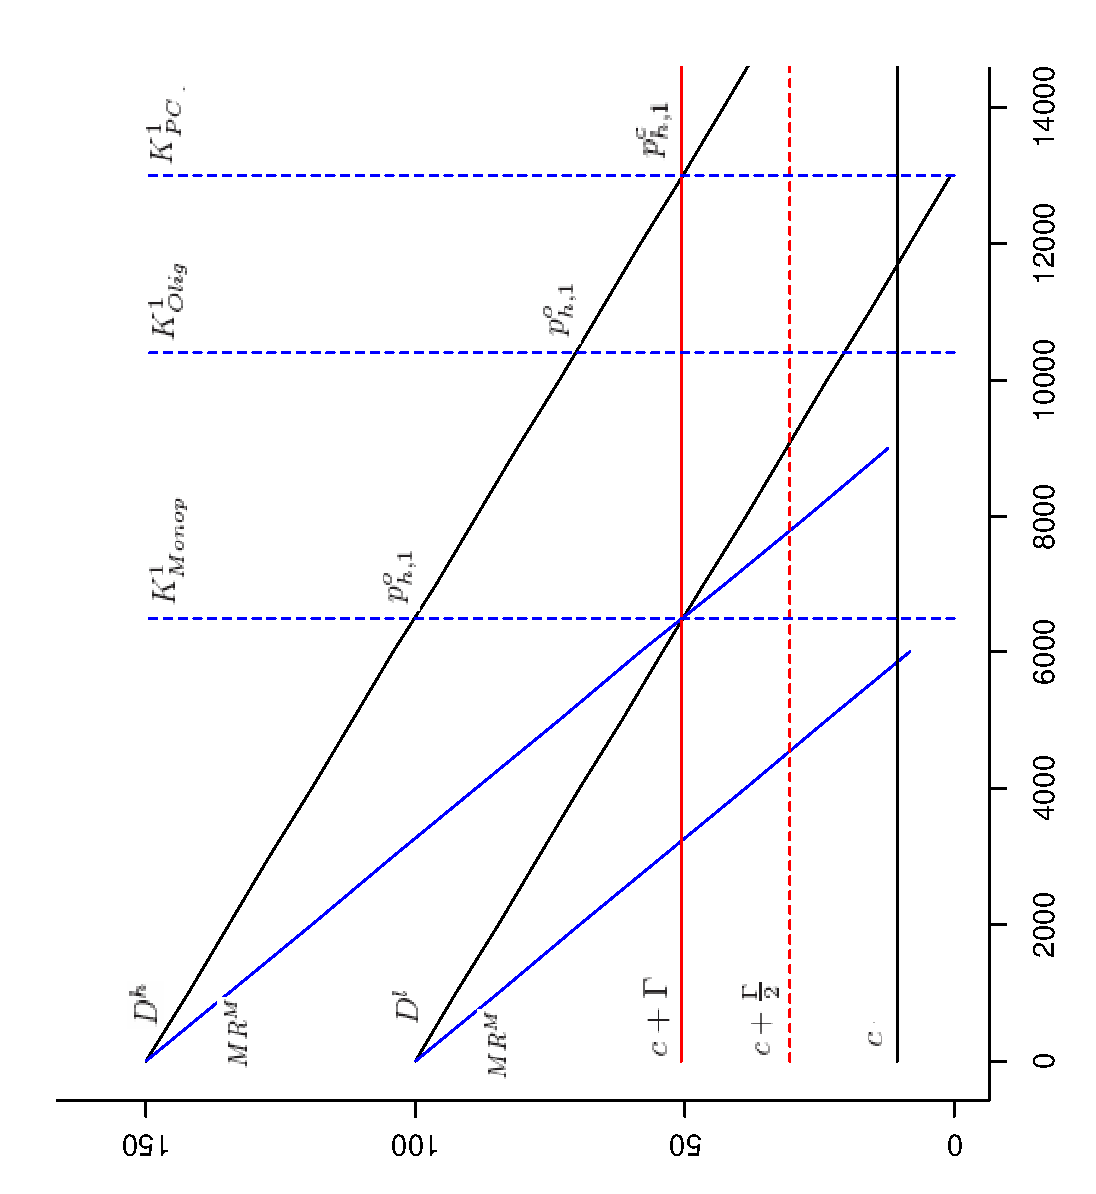
\includegraphics[width=1.0\textwidth, angle=270]{11}
    \label{fig:1}            
\end{figure}
\end{column}

\begin{column} {0.4\textwidth}

\begin{itemize}
	\item optimum
	
\begin{itemize}
	\item capacities expanded until price = LRIC ($c+ \Gamma$)
	\item $p^c_{l,1} = c$ $p^c_{h,1} = c + \lambda_{i}^{h,1}$
\end{itemize}
  \item monopoly
\begin{itemize}
  \item prices at $100$ and $55.3$
  \item but $MR = c+ \Gamma$
\end{itemize}
  \item oligopoly
  
\begin{itemize}
	 \item $MR = c+ \Gamma$ for all four players
	 \item off peak price $28.5$ - withholding
\end{itemize}
\end{itemize}
\end{column}
\end{columns}

\end{frame}


\begin{frame} {two binding periods}					
\begin{columns}
\begin{column} {0.6\textwidth}
\begin{figure}[h]
\centering
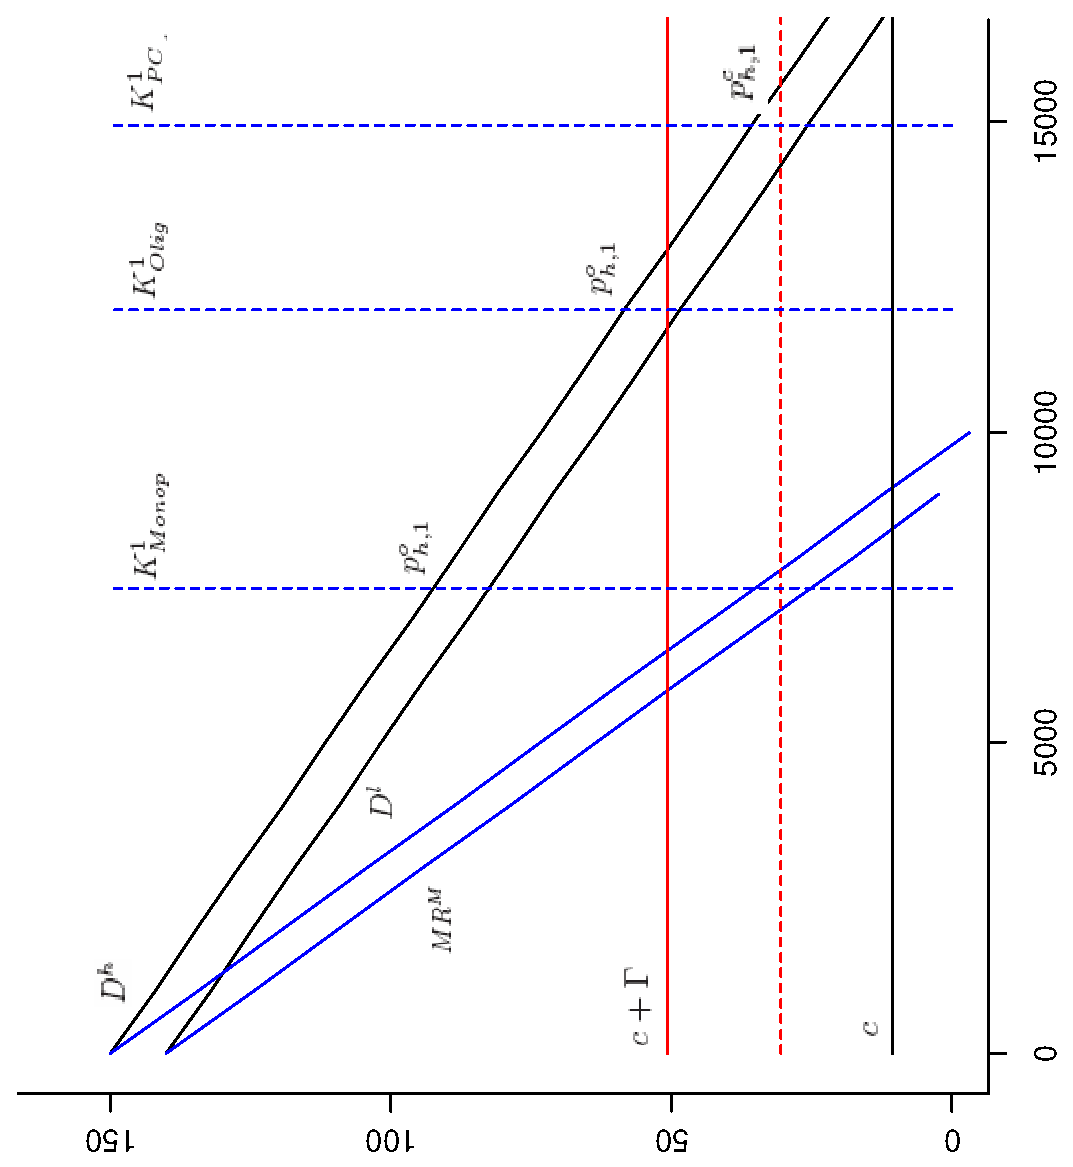
\includegraphics[width=1.0\textwidth,angle=270]{22}
    \label{fig:1}            
\end{figure}
\end{column}

\begin{column} {0.4\textwidth}

\begin{itemize}
	\item binding capacities in two periods
	\item $p^c_{h,1}$ can be far lower
	\item even lower than $c+\Gamma$
\end{itemize}

\end{column}
\end{columns}

\end{frame}

\begin{frame} {$\rho_h = \rho_l = 0.5$ competition under uncertainty}
\begin{columns}
\begin{column} {0.6\textwidth}
\begin{figure}[h]
\centering
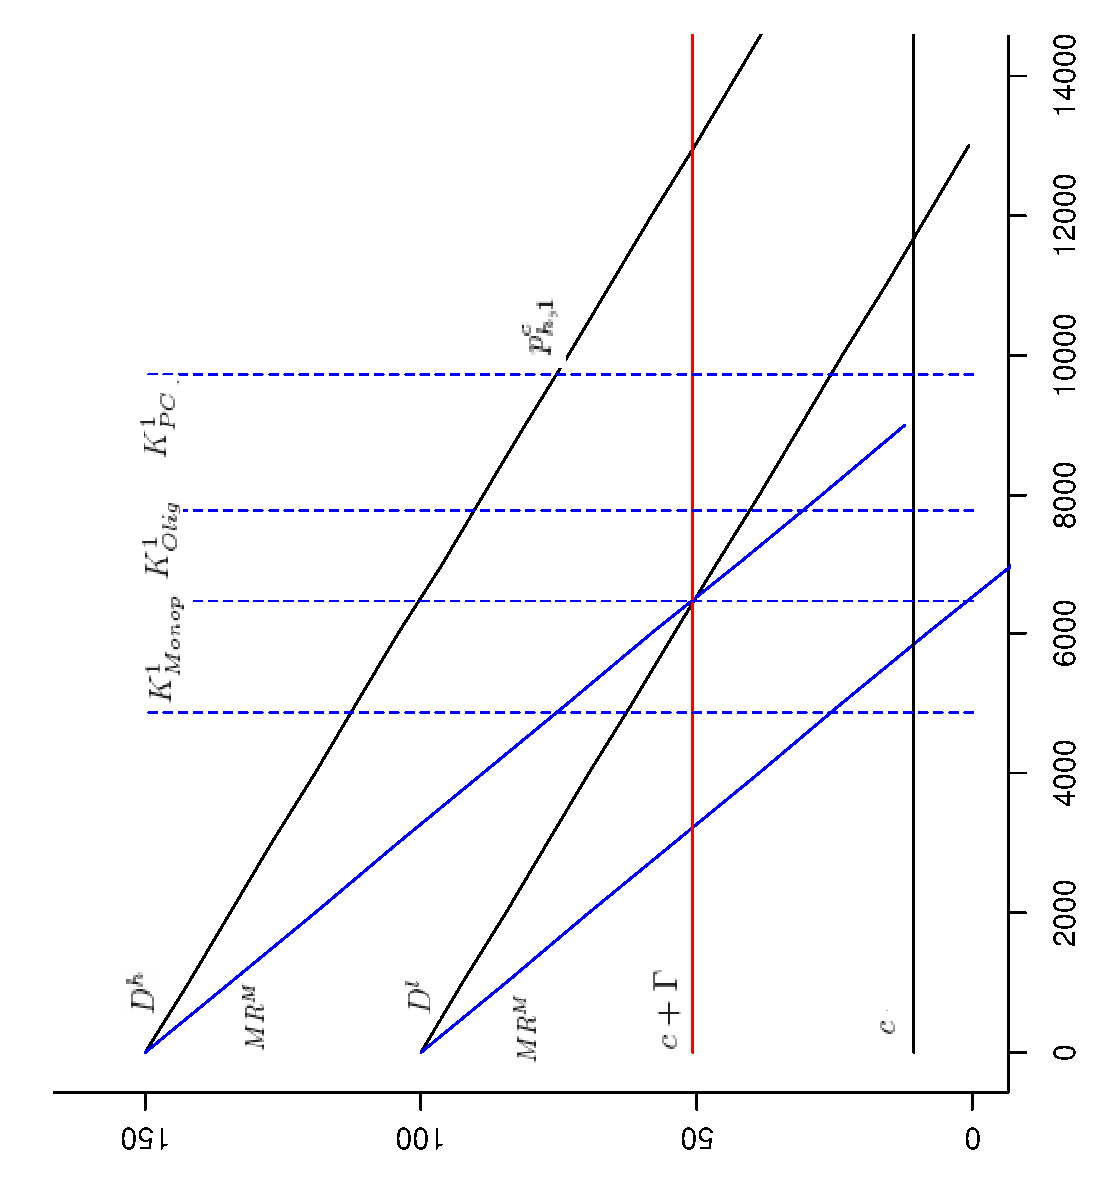
\includegraphics[width=1.0\textwidth, angle=270]{33}
    \label{fig:1}            
\end{figure}
\end{column}

\begin{column} {0.4\textwidth}



\begin{itemize}
\item as in [Gabszewicz and Poddar (1997)], investments in the stochastic solution are bigger than in the certainty equivalent game
\end{itemize}
\end{column}
\end{columns}
\end{frame}


\section{Price Caps}

\subsection{Modeling Price Caps}

\begin{frame}{Modeling Price Caps I}

\begin{gather}
	\max \pi_i(q_{i}^{s,t},K_{i}^t,I_{i}^t, \overline{p})= \label{eq:pcmax1}
	\sum_{s\in S} \rho_s \left[ ( \min{(p_{s,1}^{o},\overline{p})} - c) q_{i}^{s,1}  \right] - \Gamma I_{i}^{0}  \\
			\text{s.t.:} \  p_{s,1}^{o} - \overline{p} \leq 0; \forall s,t \label{eq:pcconstraint}
\end{gather}

\begin{itemize}
	\item oligopoly- monopoly price $p_{s,1}^{o}= \alpha^s - \beta Q^{s,1}$ may not increase beyond $\overline{p}$
	\item profit function: either oligopoly, monopoly or a fixed price $\overline{p}$ for every unit sold (non differentiable point)
	\item additional assumption: $s \in h,l$ and $\alpha^h > \alpha^l$
\end{itemize}

\end{frame}

\begin{frame}{Modeling Price Caps II}

\begin{itemize}
	\item Stage 1: solve the model without a price cap for $p_{s,1}^{o}$ and the optimal price $p_{s,1}^{c}$
	\item Stage 2: three cases \\
	case 1: if the price cap is not binding - done


\end{itemize}

\begin{table}[h]
	\centering
\begin{tabular}{ccc}
\hline
        &  case 2  & case 3  \\
\hline
        & $c+\Gamma \leq p_{h,1}^{c}$ & $c+\Gamma > p_{h,1}^{c}$ \\
\hline
\multicolumn{ 1}{c}{\textbf{a: }$\overline{p} \geq p_{h,1}^{c}$} & optimal capacities possible  & \multicolumn{ 1}{c}{not optimal} \\
\multicolumn{ 1}{c}{} & at $\overline{p} = p_{h,1}^{c}$ & \multicolumn{ 1}{c}{} \\
\hline
\multicolumn{ 1}{c}{\textbf{b:} $\overline{p} < p_{h,1}^{c}$} & \multicolumn{ 1}{c}{not optimal} & second best PC \\

\multicolumn{ 1}{c}{} & \multicolumn{ 1}{c}{} & at $c+\tfrac{\Gamma}{(\rho_h+\rho_l)}$ \\
\hline
\end{tabular}  
\end{table}

\end{frame}

\begin{frame}{Case 2a}

in interval 2a, there are no discontinuities and we can use:

\begin{gather}
	\max \pi_i(q_{i}^{s,t},K_{i}^t,I_{i}^t, \overline{p})= \label{eq:pcmax2}
	\sum_{s\in S} \rho_s \left[ (p_{s,1}^{o} - c) q_{i}^{s,1}  \right] - \Gamma I_{i}^{0}  \\  \nonumber 
\end{gather}

first order condition $\frac{\partial H}{ \partial q_{i}^{s,1}}$ changes to:

\begin{gather}
 \rho_s \left[ \alpha^s - \beta q_{i}^{s,1} - \beta Q^{s,1}\right] + \beta \psi_s =  \rho_s c  + \lambda_{i}^{s,1}   ;\ \forall i,s  \label{eq:foc1c}
\end{gather}

\begin{itemize}
	\item  $\psi_s$ is the slack variable of the PC
	\item the lower is the PC, the more quantities and thereby investments are distorted upwards
	\item PC could be set such that the left side is equal to the perfect competition result
	\item but price caps are a bold instrument
\end{itemize}
\end{frame}

\begin{frame}{Case 2b and 3}

If $\overline{p}$ is lower than $p_{s,1}^{c}$, fixed costs in peak load periods are not covered any more - missing money problem

\begin{gather}
	\max \pi_i(q_{i}^{s,t},K_{i}^t,I_{i}^t, \overline{p})= \label{eq:pcmax3}
	 \rho_h \left[ (\overline{p}-c) q_{i}^{l,1}  \right]+ \rho_h \left[ (p_{l,1}^{o} - c) q_{i}^{l,1}  \right] - \Gamma I_{i}^{0}  \\  \nonumber
\end{gather}

$\overline{p}-c$ can now be seen as a mere subsidy a firm considers when deciding on how much capacity should be built for the off peak period

\end{frame}

\subsection{Numerical Solutions}

\begin{frame} {Case 2a and 2b}
					
\begin{columns}
\begin{column} {0.6\textwidth}
\begin{figure}[h]
\centering
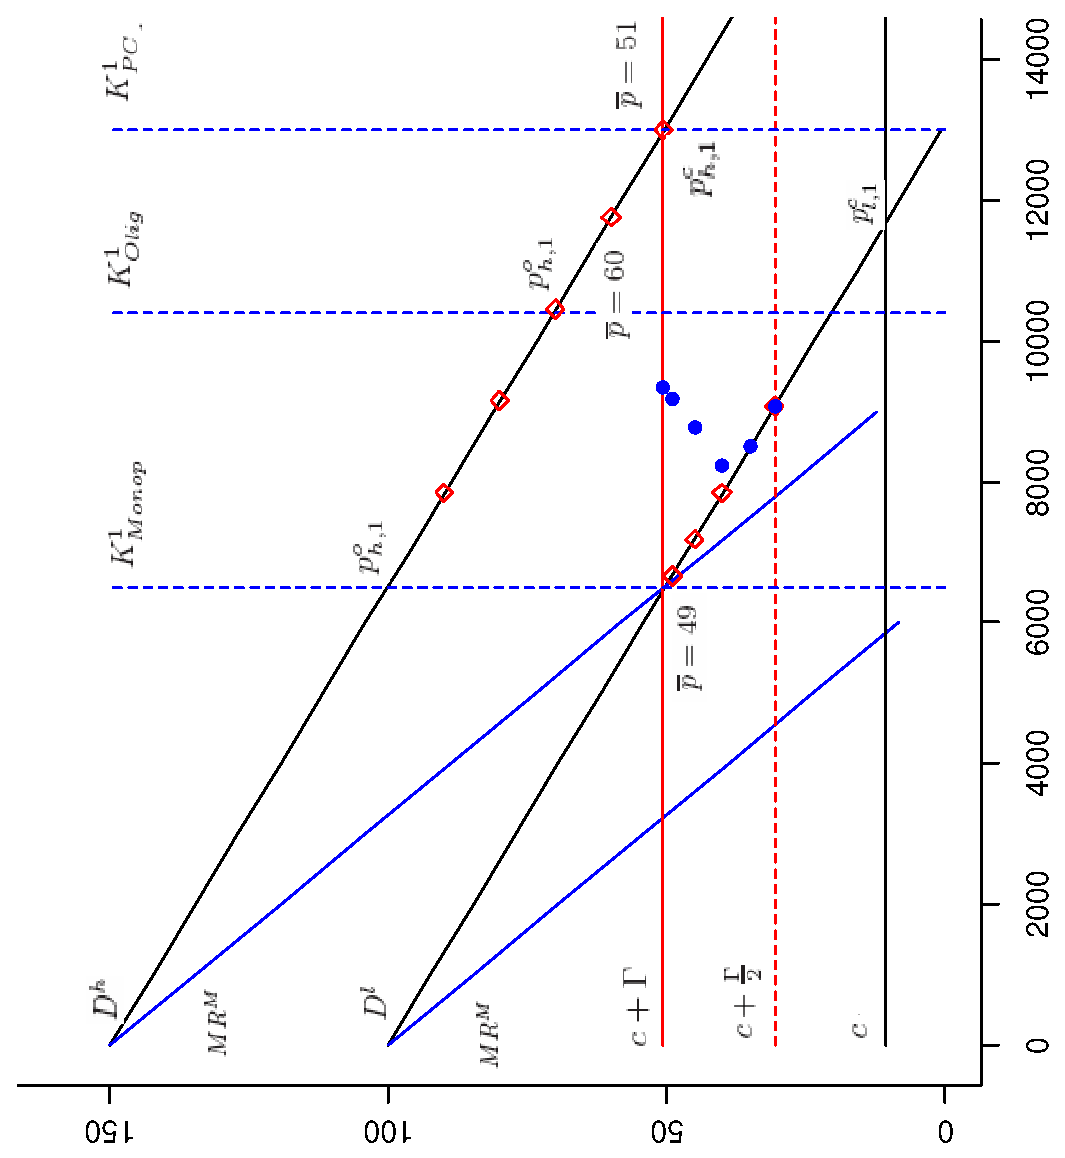
\includegraphics[width=1.0\textwidth, angle=270]{44}
    \label{fig:1}            
\end{figure}
\end{column}

\begin{column} {0.4\textwidth}
2a:
\begin{itemize}
	\item every additional unit yields $\overline{p}- c -\Gamma$
	\item no incentive for strategic investment withholding any more
	\item $\overline{p} = p_{s,1}^{c}$ optimal PC
\end{itemize}
2b:
\begin{itemize}
	\item different solutions for monopoly and oligopoly case
	\item $c+\tfrac{\Gamma}{(\rho_h+\rho_l)}$ lowest possible PC
\end{itemize}

\end{column}
\end{columns}
\end{frame}


\begin{frame} {Case 2a and 2b under Uncertainty}					
\begin{columns}
\begin{column} {0.6\textwidth}
\begin{figure}[h]
\centering
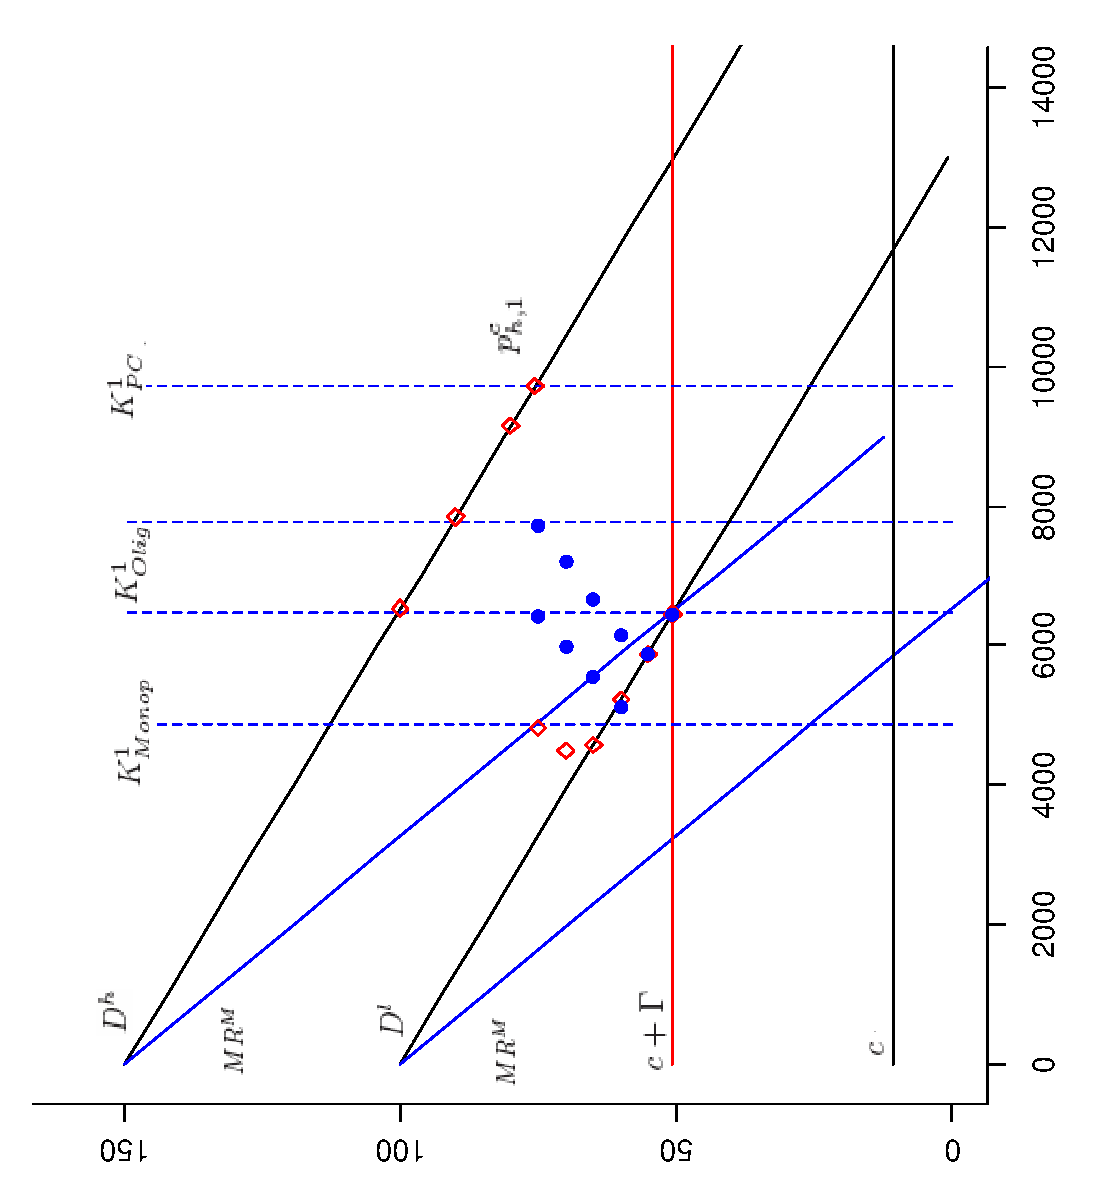
\includegraphics[width=1.0\textwidth, angle=270]{55}
    \label{fig:1}            
\end{figure}
\end{column}

\begin{column} {0.4\textwidth}

\begin{enumerate}
	\item $\overline{p}$ is not binding if demand is low
	\item the monopolist reduces investments, until he has sufficient investment incentives again
\end{enumerate}

\end{column}
\end{columns}
\end{frame}

\begin{frame} {Case 3}					
\begin{columns}
\begin{column} {0.6\textwidth}
\begin{figure}[h]
\centering
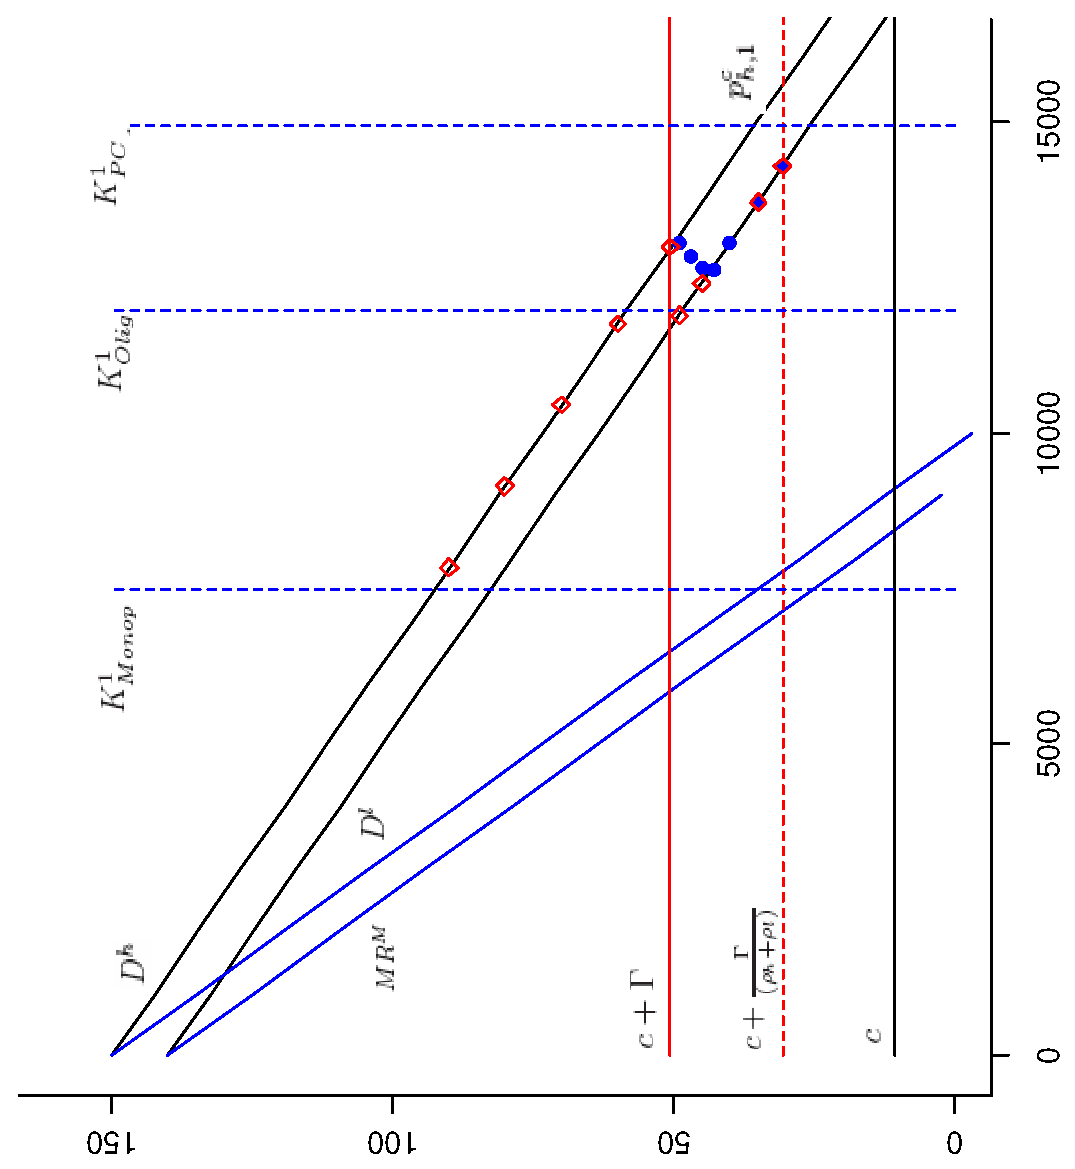
\includegraphics[width=1.0\textwidth, angle=270]{66}
    \label{fig:1}            
\end{figure}
\end{column}

\begin{column} {0.4\textwidth}

\begin{itemize}
	\item optimal investments cannot be obtained by price caps
	\item second best optimum at $c+\tfrac{\Gamma}{(2)}$
\end{itemize}

\end{column}
\end{columns}

\end{frame}

\section{Conclusion}


\begin{frame} {Conclusion}					


\begin{itemize}
	\item we modeled the optimal behavior of firms in a two stage investment game under uncertainty and a peak load pricing cost structure
	\item we compared the monopoly, oligopoly and perfect competition case
	\item in some cases it is possible to reach an optimal level of capacity investments
	\item risks attached to price caps - "`missing money problem"'
	\item price caps require a lot of information
\end{itemize}

\begin{alertblock}{main messages}
\begin{itemize}
	 \item there are incentives for strategic investment withholding
	 \item prices can increase investment incentives but are risky if set wrong
\end{itemize}
\end{alertblock}

\end{frame}
\begin{frame}{Tree}
\begin{center}
\psscalebox{0.60}{
\psset{nodesep=0pt,labelsep=1pt,nrot=:U}
\psmatrix[colsep=3.0cm,rowsep=0.0cm] 
                               &                                    &                                       & \circlenode{H}{$n_7$}\\ 
                               &                                    & \circlenode{D}{$n_3$}\\  
                               &                                    &                                       & \circlenode{I}{$n_8$}\\              
                               &  \circlenode{B}{$n_1$} & & \\
                               &                                    &                                       & \circlenode{J}{$n_9$}\\ 
                               &                                    & \circlenode{E}{$n_4$}\\  
                               &                                    &                                       & \circlenode{K}{$n_{10}$}\\ 
    \circlenode{A}{$n_0$} &                          &              & \\
                               &                                    &                                       & \circlenode{L}{$n_{11}$}\\ 
                               &                                    & \circlenode{F}{$n_5$}\\  
                               &                                    &                                       & \circlenode{M}{$n_{12}$}\\              
                               &  \circlenode{C}{$n_2$} & & \\
                               &                                    &                                       & \circlenode{N}{$n_{13}$}\\ 
                               &                                    & \circlenode{G}{$n_6$}\\  
                               &                                    &                                       & \circlenode{O}{$n_{14}$}\\ 
& & & \\
 $t=0$ & $t = 1$ & $t=2$ &  $t=3$\\
\ncline[linewidth=1.5pt]{A}{B}\naput{$50\%$}
\ncline[linewidth=1.5pt]{A}{C}\naput{$50\%$}
\ncline[linewidth=1.5pt]{B}{D}\naput{$25\%$}
\ncline[linewidth=1.5pt]{B}{E}\naput{$25\%$}
\ncline[linewidth=1.5pt]{C}{F}\naput{$25\%$}
\ncline[linewidth=1.5pt]{C}{G}\naput{$25\%$}
\ncline[linewidth=1.5pt]{D}{H}\naput{$12.5\%$}
\ncline[linewidth=1.5pt]{D}{I}\naput{$12.5\%$}
\ncline[linewidth=1.5pt]{E}{J}\naput{$12.5\%$}
\ncline[linewidth=1.5pt]{E}{K}\naput{$12.5\%$}
\ncline[linewidth=1.5pt]{F}{L}\naput{$12.5\%$}
\ncline[linewidth=1.5pt]{F}{M}\naput{$12.5\%$}
\ncline[linewidth=1.5pt]{G}{N}\naput{$12.5\%$}
\ncline[linewidth=1.5pt]{G}{O}\naput{$12.5\%$}
\endpsmatrix}
\end{center}
\end{frame}

\begin{frame}{Notation}
  \begin{tabular}[l]{l l}
\centering
$i \in \mathcal{I}$ & players, firms \\
$j \in \mathcal{J}$ & available technologies \\
$m\in\mathcal{M}$ & market states \\
$p_n$ & probability to reach a certain node\\
$p^m$ & probability of market state $m$ \\
$ q_{i,n}^{j,m}$ & production quantities \\
$I_{i,n}^{j}$ & investment quantities, for $n\in\left\{n_0\right\}\cup\mathcal{T}$ \\
$K_{i,n}^{j}$ & available capacity\\
$F_n^{j}$ & investment cost\\
$P^m_n = \alpha_n^m-\beta^m\sum_{i\in \mathcal{I}}\sum_{j\in \mathcal{J}}q_{i,n}^{j,m}$ & market equilibrium price \\
$\alpha_n^m$ & intercept of demand function \\
$\beta^m$ & slope of demand function \\
$c_j$ & variable costs \\
$\delta_n$ & discount factor \\
$\nu$ & salvage value parameter\\
$\rho$ & depreciation rate\\
\end{tabular}
\end{frame}

\begin{frame}{Optimization}

\begin{equation}
  \label{eq:objfct}
  \max_{q_{i,n}^{j,m}, I_{i,n}^{j}} \sum_{n\in \mathcal{N}}p_n\delta_n\Pi_{i,n}\left(q_{i,n}^{j,m}, I_{i,n}^{j}, K_{i,n}^{j}, Q_n^m\right)+ \sum_{n\in \mathcal{S}}p_n\,\delta_n \sum_{j\in \mathcal{J}}K_{i,n}^{j}F_n^{j}\nu
\end{equation}
subject to
  
\begin{eqnarray}  
q_{i,n}^{j,m} - K_{i,n}^{j} &\leq& 0 \quad \forall i,j,m,n \label{eq:prodconstr} \\
Q_n^m-\sum_{i\in \mathcal{I}}\sum_{j\in \mathcal{J}} q_{i,n}^{j,m} &=& 0 \quad \forall m,n \label{eq:marketclearing}\\
K_{i,n}^{j} - (1-\rho)K_{i,a(n)}^{j}-I_{i,a(n)}^{j} &=& 0 \quad \forall i,j,n \label{eq:state} \\
q_{i,n}^{j,m}, K_{i,n}^{j}, I_{i,n}^{j}, Q_n^m  &\geq& 0 \quad \forall i,j,m,n\label{eq:nonneg}
\end{eqnarray}
  
\end{frame}



\section{The German Electricity Market}

\subsection{Installed capacities}

\begin{frame}{Installed capacities}
					
\begin{figure}[h]
  \centering
%\caption{Installed capacities in GW of major players in Germany}
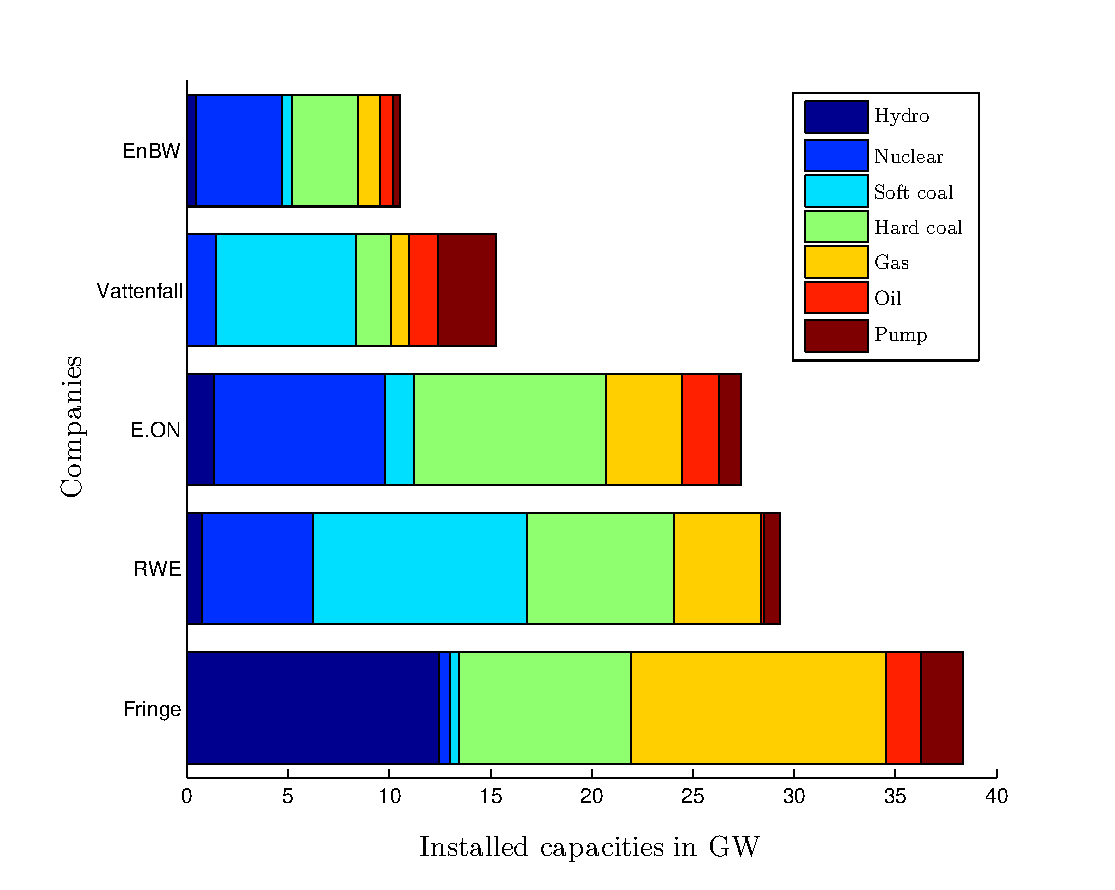
\includegraphics[width=0.8\textwidth]{capacities}
  \label{fig:capacities}
\\
\vspace{0.1cm}
\scriptsize Source: International Energy Agency (2007)
\end{figure}

\end{frame}

\subsection{Electricity load and prices}

\begin{frame} {Electricity load}
					
\begin{figure}[h]
\centering
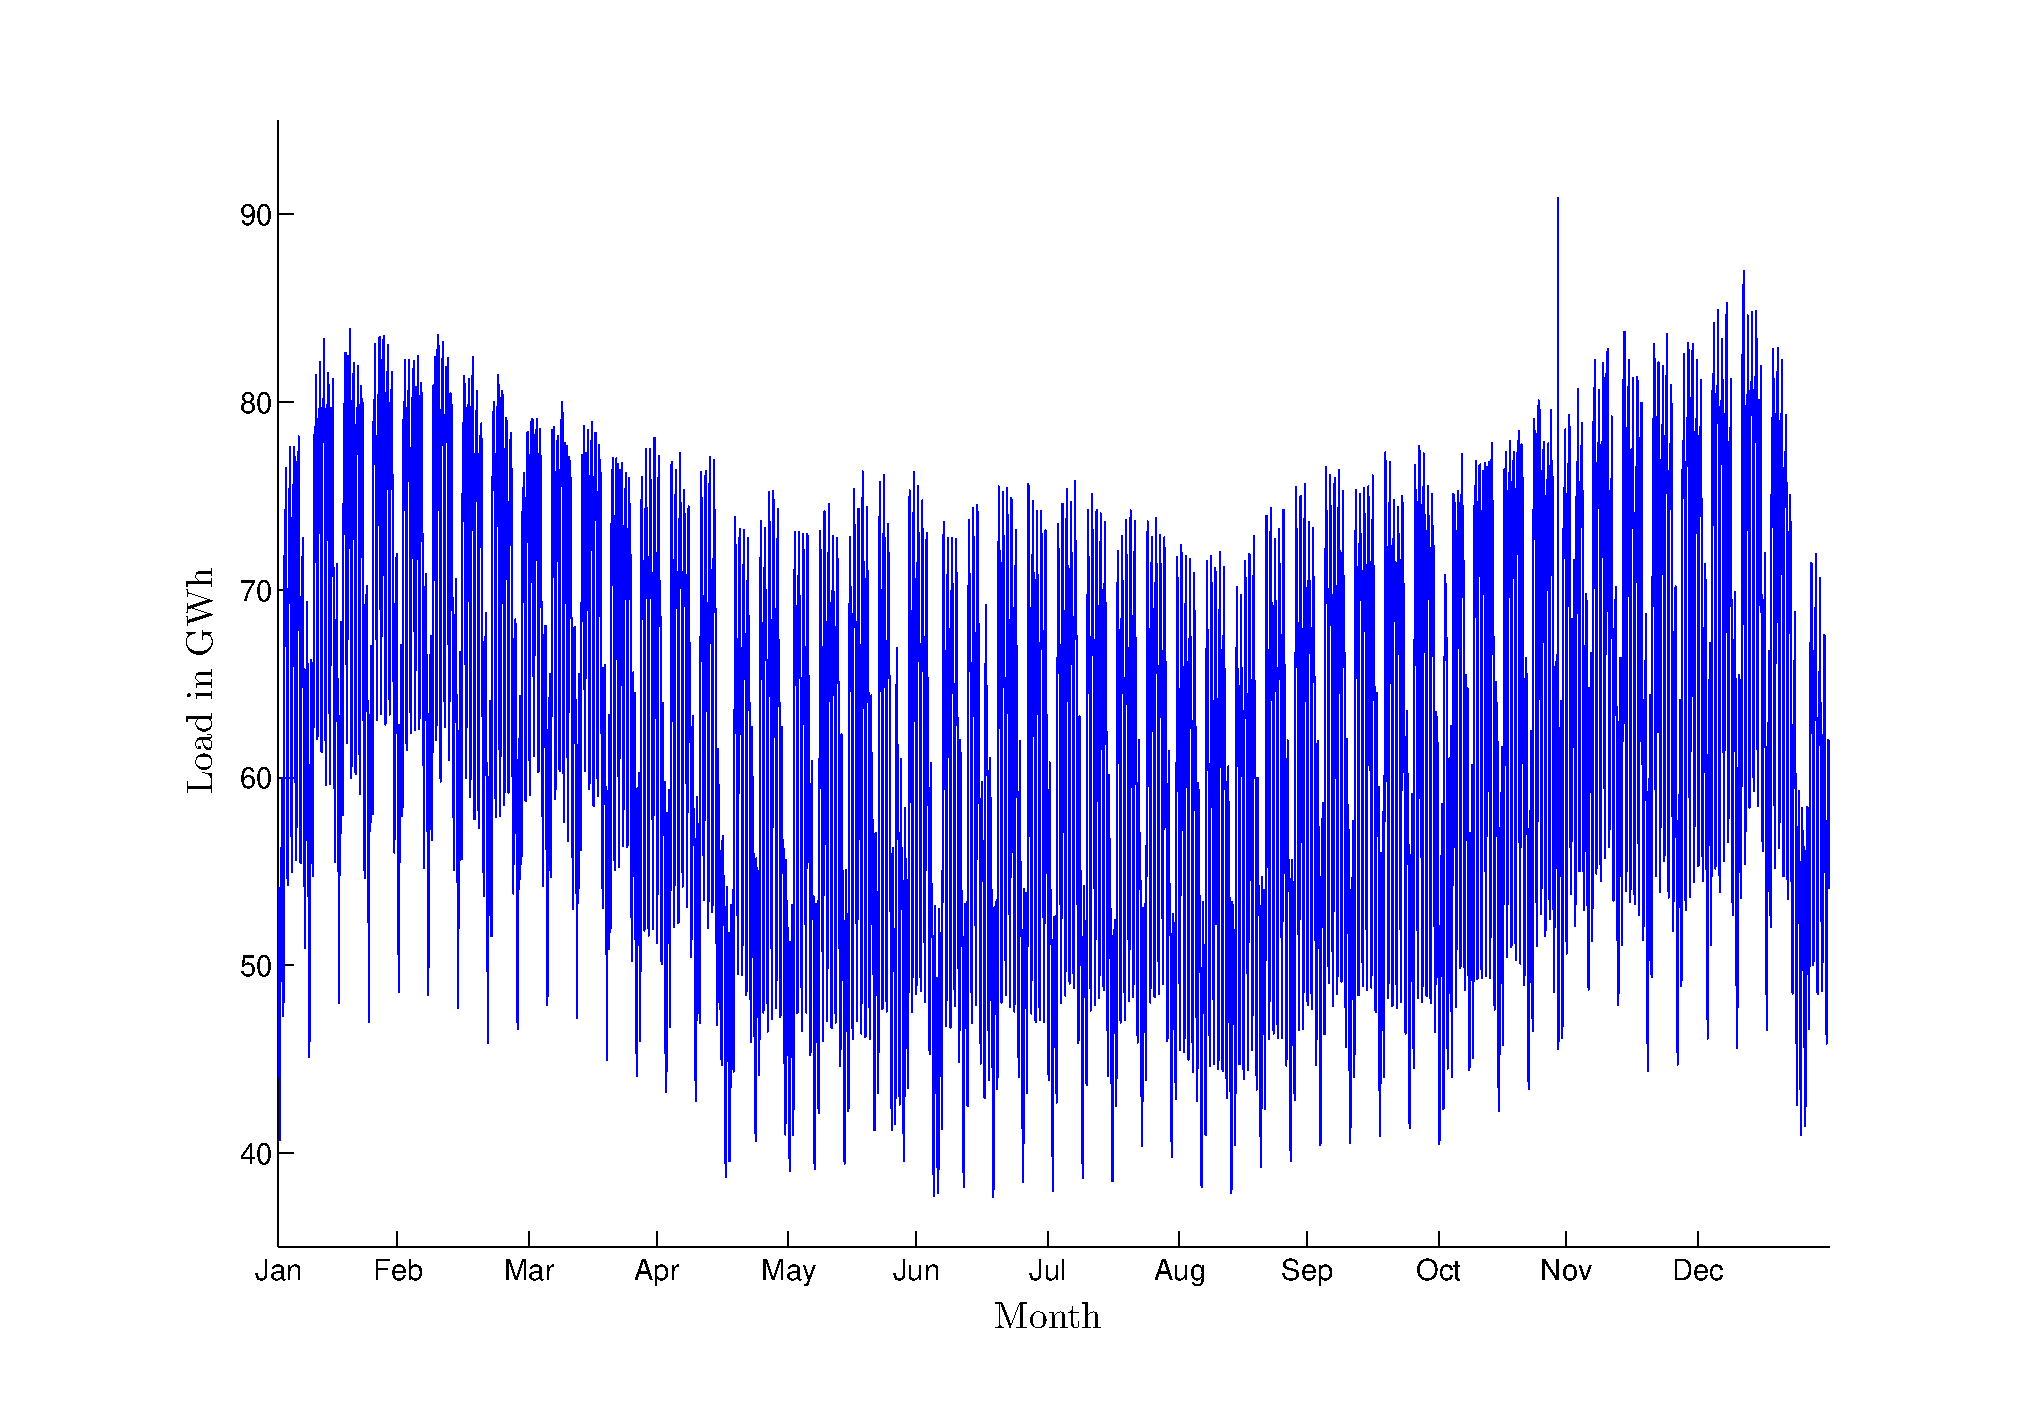
\includegraphics[width=0.9\textwidth, angle=0]{loadvalues}
    \label{fig:load}   
\\ 
\vspace{0.1cm}
\scriptsize Source: UCTE (2006)           
\end{figure}
\end{frame}

\begin{frame} {Electricity prices}				
\begin{figure}[h]
\centering
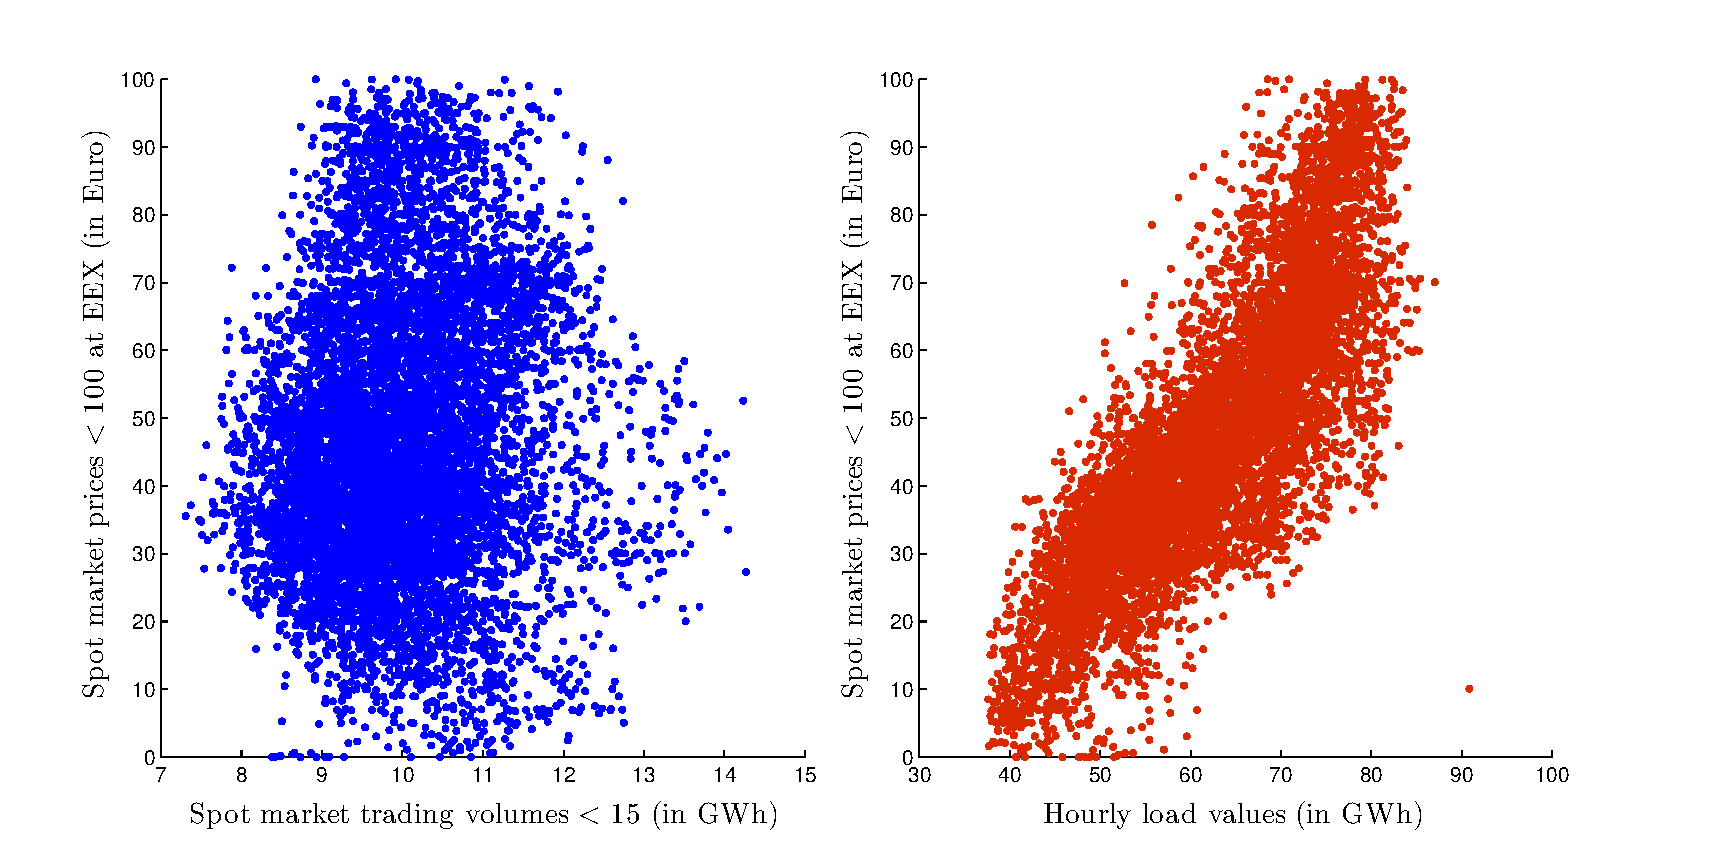
\includegraphics[width=1.0\textwidth, angle=0]{pricequant}
    \label{fig:load} 
\\ 
\vspace{0.1cm}
\scriptsize Source: EEX (2006); UCTE (2006)           
\end{figure}
\end{frame}

\begin{frame}
  \frametitle{Market segments}

\begin{center}
\small
\begin{tabular}{rrrrr}
  \hline
Price & Average price  & Average quantity & Number of & Percentage of \\
intervals& (Euro/MWh) &  (MWh) &  prices & of total prices\\
  \hline\hline
$0\leq p<20$ & 12.67 & 46,111.63 & 611 & 6.98\% \\
$20\leq p<40$ & 31.35 & 54,103.50 & 3,003 & 34.28\% \\
$40\leq p<60$ & 49.00 & 64,806.04 & 2,626 & 29.98\% \\
$60\leq p<80$ & 68.46 & 72,385.56 & 1,588 & 18.13\% \\
$80\leq p<100$ & 88.40 & 75,991.21 & 665 & 7.59\% \\
$100\leq p<\infty$& 176.06 & 76,482.34 & 266 & 3.04\% \\
   \hline
\end{tabular}  
\normalsize
\end{center}

\end{frame}

\subsection{Marginal and investment costs}

\begin{frame}
  \frametitle{Marginal and investment costs}
\begin{center}
  \begin{tabular}{rrr}
\hline
           & Variable costs & Investment costs\\
           &  (Euro/MWh)    &  (Euro/GW) \\
\hline\hline
     Hydro &        7.6 &    3,500\\

   Nuclear &        9.5 &    1,841 \\

   Lignite &       10.6 &    1,074 \\

 Hard coal &       16.1 &     971 \\

 Gas (CCGT) &       33.5 &     460 \\

Oil & 44            &   n/a\\

Pump &         80 &       n/a\\
\hline
\end{tabular}
\\
\vspace{0.3cm}
\scriptsize Source: Auer et al. (2006)
\end{center}
\end{frame}

\section{Results}

\subsection{Scenario generation}

\begin{frame}
  \frametitle{Scenario generation}
\begin{figure}[h]
  \centering
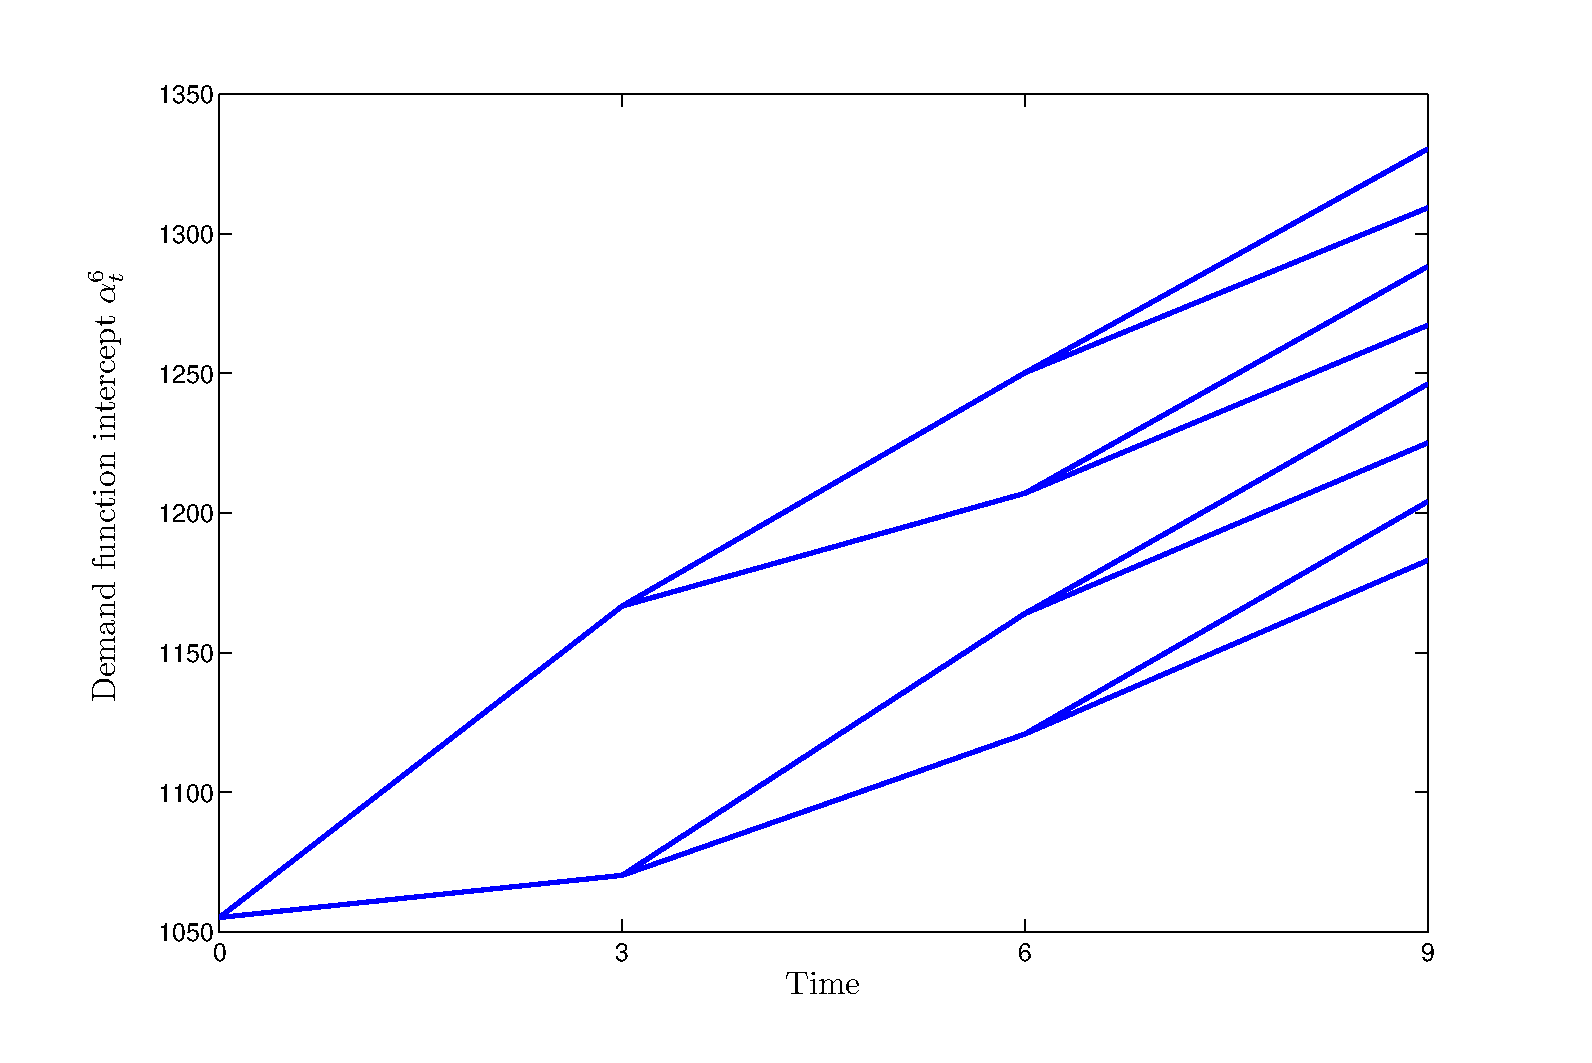
\includegraphics[width=1\textwidth]{intercept}
  \label{fig:intercept}
\end{figure}  
\end{frame}


\subsection{Solution of the MCP}

\begin{frame}
  \frametitle{Production in the initial node $q_{i,0}^{m}$ (in MWh)}
  \begin{center}
\scriptsize
      \begin{tabular}{rrrrrrr}
\hline
           &     $m=1$ &     $m=2$ &     $m=3$ &     $m=4$ &     $m=5$ &     $m=6$ \\
\hline\hline
       Rwe &    10,945.21  &    13,590.03  &    17,150.64  &    20,586.19  &    21,872.07  &    21,984.52  \\

       EON &    10,945.21  &    13,592.14  &    17,150.64  &    20,586.09  &    21,871.99  &    21,984.48  \\

    Vattenfall &    10,940.85  &    13,590.03  &    15,273.00  &    15,273.00  &    15,273.00  &    15,273.00  \\

      EnBW &    10,528.00  &    10,528.00  &    10,528.00  &    10,528.00  &    10,528.00  &    10,528.00  \\
\hline
\end{tabular}
\normalsize
  \end{center}
\end{frame}



\begin{frame}
  \frametitle{Sensitivity analysis}

  \begin{itemize}
  \item Investment quantities in the initial node $I_{i,0}$ (in MW) with $\rho=0.025$
  \end{itemize}

\begin{center}
  \begin{tabular}{rrrrr}
\hline
           &       $\nu=0.99$ &       $\nu=0.95$ &        $\nu=0.9$ &       $\nu=0.85$ \\
\hline\hline
 Vattenfall  &      5,015.93  &      4,832.23  &      4,626.18  &      4,516.54  \\

     EnBW  &      9,582.64  &      9,405.55  &      9,229.64  &      9,120.00  \\
\hline
\end{tabular}
\end{center}

\begin{itemize}
\item Investment quantities in the initial node $I_{i,0}$ (in MW) with $\nu=0.95$
\end{itemize}

\begin{center}
  \begin{tabular}{rrrrr}
\hline
           &      $\rho=0.025$ &       $\rho=0.03$ &      $\rho=0.035$ &       $\rho=0.04$ \\
\hline\hline
Vattenfall &      4,832.23  &      4,908.60  &      4,984.96  &      5,061.33  \\

      EnBW &      9,405.55  &      9,458.19  &      9,510.83  &      9,563.47  \\
\hline
\end{tabular}  
\end{center}

\end{frame}

\section{Conclusion}


\begin{frame} {Conclusion}					


\begin{itemize}
	\item we modeled the optimal behavior of firms in a two stage investment game under uncertainty and a peak load pricing cost structure
	\item we compared the monopoly, oligopoly and perfect competition case
	\item we calibrated the model with real world data
	\item quantify investment potentials
\end{itemize}

\begin{alertblock}{main messages}
\begin{itemize}
	 \item there are incentives for strategic capacity and investment withholding
	 \item price caps can increase investment incentives but are risky due to the "missing money problem"
\end{itemize}
\end{alertblock}

\end{frame}






\begin{frame}
\frametitle{Literature}
\begin{thebibliography}{PLP}

\bibitem[Boom and B�hler (2007)]{Boom2007}
Boom and B�hler (2007).
\newblock Restructuring Electricity Markets when Demand is Uncertain: Effects on Capacity Investments, Prices and Welfare
\newblock {\em University of Copenhagen. Department of Economics. Centre for Industrial Economics. WP 2007-09}.

\bibitem[Cramton and Stoft (2006)]{Cramton2006}
Cramton and Stoft (2006).
\newblock The Convergence of Market Designs for Adequate Generating Capacity with special Attention to the CAISO�s Resource Adequacy Problem.
\newblock {\em Center for Environmental Policy Research}.

\bibitem[Crew and Kleindorfer (1986)]{Crew1986}
Crew and Kleindorfer (1986).
\newblock The Economics of Public Utility Regulation
\newblock {\em London: Mc Millan Press}.

\bibitem[Ferris and Munson (2000)]{Ferris2000}
Ferris and Munson (2000).
\newblock Complementarity Problems in GAMS and the PATH Solver
\newblock {\em Journal of Economic Dynamics and Control}.
\end{thebibliography}

\end{frame}

\begin{frame}
\frametitle{Literature II}

\begin{thebibliography}{PLP}

\bibitem[Gabszewicz and Poddar (1997)]{Gabszewicz1997}
Gabszewicz and Poddar (1997).
\newblock Demand fluctuations and capacity utilization under duopoly.
\newblock {\em Economic Theory, 10, 131-146}.

\bibitem[Genc, Reynolds and Sen (2007)]{Genc2007}
Genc, Reynolds and Sen (2007)
\newblock Dynamic Oligopolistic Games under Uncertainty: A Stochastic Programming Approach.
\newblock {\em Journal of Economic Dynamics and Control}.

\bibitem[Joskow and Tirole (2007)]{Joskow2007}
Joskow and Tirole (2007)
\newblock Reliability and competitive electricity markets.
\newblock {\em The Rand Journal of Economics}.

\bibitem[Kreps and Scheinkman (1983)]{Kreps1983}
Kreps and Scheinkman (1983).
\newblock Quantity precommitment and bertrand competition yields cournot outcomes.
\newblock {\em Bell Journal of Economics 14}.

\end{thebibliography}
\end{frame}

\begin{frame}
\frametitle{Literature III}

\begin{thebibliography}{PLP}

\bibitem[Genc, Reynolds and Sen (2007)]{Genc2007}
Genc, Reynolds and Sen (2007)
\newblock Dynamic Oligopolistic Games under Uncertainty: A Stochastic Programming Approach.
\newblock {\em Journal of Economic Dynamics and Control}.

\bibitem[Murphy and Smeers (2005)]{Murphy2005}
Murphy and Smeers (2005)
\newblock Generation Capacity Expansion in Imperfectly Competitive Restructured Electricity Markets.
\newblock {\em Operations Research}.

\bibitem[Roques and Savva (2006)]{Roques2006}
Roques and Savva (2006)
\newblock Price cap regulation and investment incentives under demand uncertainty.
\newblock {\em CWPE 0636 and EPRG 0616 Working Paper.}.

\end{thebibliography}
\end{frame}

\end{document}